\documentclass[11pt]{article}

\usepackage{a4wide}
\usepackage[francais]{babel}
\usepackage[utf8x]{inputenc}
\usepackage{graphicx}
\usepackage{subcaption}

\begin{document}


\title{Projet Recherche Documentaire}



\begin{center}


\Huge M1 Informatique \\
\vspace{3cm}
Projet Recherche Documentaire\\

Méthode vectorielle \LARGE
\end{center}






\vspace{15cm}
Cyril Lepinette \\
Romain Grelier

\pagebreak

\section{Introduction}
Dans le cadre de l'UE "Recherche Documentaire" nous avons implémenté un programme de recherche de document en évaluant la pertinence de ceux-ci en fonction d'une requête envoyée par l'utilisateur.
Dans ce document nous décrivons le pipeline utilisé pour l'indexation des documents et le traitement des requêtes.

\section{Traitement des fichiers}

\subsection{Lecture des fichiers}
Les textes constituant le corpus sont dans plusieurs fichiers qui contiennent les textes des documents aussi plusieurs autres données, comme le titre, des notes ...
Ces données doivent donc être récupérée à l'aide d'un lecteur de fichier.

Les fichiers utilisent un language de balise qui vont nous servir à la lecture de celui-ci, les balises qui vont nous intérésser sont les balises "DOCNO" et "TEXT".
Le lecteur est capable de gérer la plupart de ces balises, lors de la lecture, les données sont regroupées par document et stocké dans un objet python "Document".

\subsection{Suppression des caractères spéciaux}
Une fois les fichiers lu et stockés, nous observons des caractères qui ne seront pas forcement utile comme la ponctuation, dans notre implémentation nous avons choisit de les supprimer.
La suppression de ces caractères se fait à l'aide d'une expression régulière pour la ponctuation et les chiffres.

\subsection{Racinisation (Stemming)}
Le Stemming permet de trouver la racine des mots pour des recherches plus efficace, nous avons utiliser une implémentation existante appelée Porter Stemming (voir source).

\subsection{Index inversé}
L'index inversé est l'ensemble des mots présents dans le corpus qui réfère aux textes qui les contiennent après être passé par les étapes de suppression des caractères spéciaux et de stemming.
L'index des implémenté sous forme d'un dictionnaire python dont la clé est le mot et la valeur est une list contenant en première position le nombre d'occurence du mot dans tout le corpus puis des tuples donnant l'index du document et le nombre d'occurrence dans celui-ci.

\pagebreak
\section{Moteur de recherche}

\subsection{Fréquence des termes et des documents (TF*IDF)}
La fréquence du terme multiplié par l'inverse de la fréquence des documents, couramment abrégé en TF-IDF consiste a calculer l'importance d'un terme dans un document contenu dans un corpus. 
\\La fréquence du terme est son nombre d'occurence dans le document. Afin de ne pas avoir un résultat trop élevé la fréquence est diminuée grâce à une fonction logarithmique. \\
La fréquence inverse de document quant à elle mesure de l'importance du terme dans l'ensemble du corpus. \\
Lorsque l'on multiplie les deux on obtient donc un résultat permettant de conclure sur l'importance d'un terme dans un document, mais relativement à l'ensemble des documents.

\subsection{Vectorisation et normalisation des documents}
La vectorisation des documents permet de créer un espace vectoriel dont les axes sont caractérisés par les termes. Les documents sont représentés par des vecteurs.  \\
Les vecteurs sont constitués des TF*IDF de tous les mots du document. \\
Un exemple pourrait être : vecteur = [1.3,0,0.1]
\begin{center}
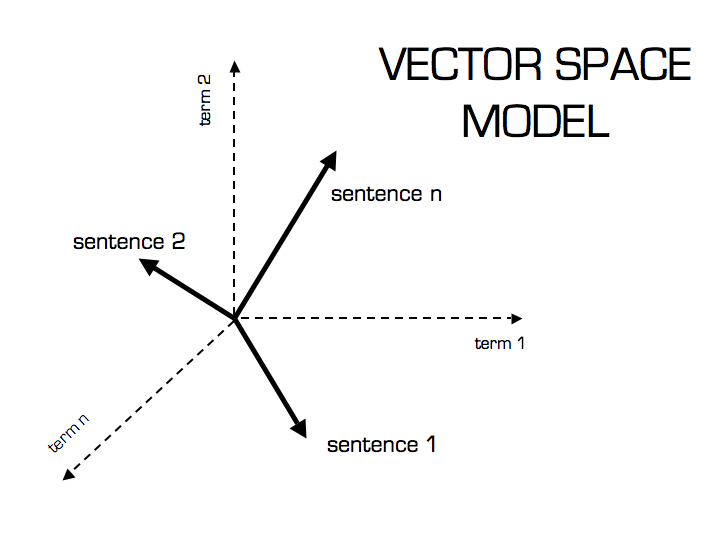
\includegraphics[scale=0.45]{vector_space}
\end{center}
\subsection{Pertinence des documents par similarité de cosinus}
La comparaison par similarité de cosinus est la dernière étape. Elle permet de comparer l'angle entre deux vecteurs et ainsi en donner la similarité. 

\begin{center}
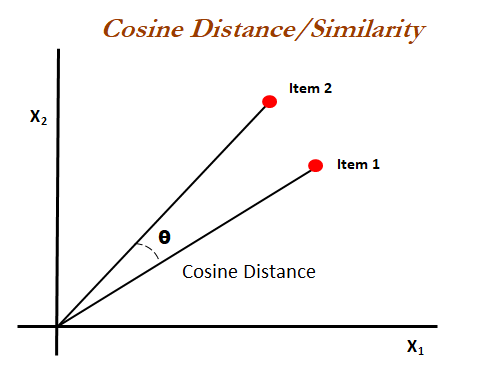
\includegraphics[scale=0.9]{cosinus}
\end{center}

\subsection{Traitement de la requête et comparaison avec le corpus}
Afin de traiter la pertinence des documents nous utilisons une méthode consistant à comparer la similarité des cosinus entre deux documents. 
La requête doit donc être transformée en document afin de pouvoir la comparer par la suite avec le corpus. 
Pour ce, nous créons un nouveau document ayant pour texte la requête. Nous le passons ensuite dans un algorithmes de racinisation. 

\pagebreak
\section{Interface graphique}
Afin de fournir une interface pouvant fonctionner sur un maximum de plateforme ainsi permettant d'être développée rapidement, c'est une interface web qui a été choisit.
C'est à l'aide du framework web Flask que nous avons implémenté l'interface, elle peut être lancée facilement, et se trouve dans le navigateur web de l'utilisateur.

Un champ de recherche permet de taper une requête et en réponse, le programme renvoit la liste des documents les plus pertinent trouvés. 

\pagebreak

\begin{thebibliography}{9}

    \bibitem{Porter_Stemming}
    The Porter stemming algorithm
    \\\texttt{http://snowball.tartarus.org/algorithms/porter/stemmer.html}

\end{thebibliography}

\end{document}